\documentclass[12pt,reqno,final,pdftex]{amsart}\usepackage[]{graphicx}\usepackage[]{color}
%% maxwidth is the original width if it is less than linewidth
%% otherwise use linewidth (to make sure the graphics do not exceed the margin)
\makeatletter
\def\maxwidth{ %
  \ifdim\Gin@nat@width>\linewidth
    \linewidth
  \else
    \Gin@nat@width
  \fi
}
\makeatother

\definecolor{fgcolor}{rgb}{0.345, 0.345, 0.345}
\newcommand{\hlnum}[1]{\textcolor[rgb]{0.686,0.059,0.569}{#1}}%
\newcommand{\hlstr}[1]{\textcolor[rgb]{0.192,0.494,0.8}{#1}}%
\newcommand{\hlcom}[1]{\textcolor[rgb]{0.678,0.584,0.686}{\textit{#1}}}%
\newcommand{\hlopt}[1]{\textcolor[rgb]{0,0,0}{#1}}%
\newcommand{\hlstd}[1]{\textcolor[rgb]{0.345,0.345,0.345}{#1}}%
\newcommand{\hlkwa}[1]{\textcolor[rgb]{0.161,0.373,0.58}{\textbf{#1}}}%
\newcommand{\hlkwb}[1]{\textcolor[rgb]{0.69,0.353,0.396}{#1}}%
\newcommand{\hlkwc}[1]{\textcolor[rgb]{0.333,0.667,0.333}{#1}}%
\newcommand{\hlkwd}[1]{\textcolor[rgb]{0.737,0.353,0.396}{\textbf{#1}}}%

\usepackage{framed}
\makeatletter
\newenvironment{kframe}{%
 \def\at@end@of@kframe{}%
 \ifinner\ifhmode%
  \def\at@end@of@kframe{\end{minipage}}%
  \begin{minipage}{\columnwidth}%
 \fi\fi%
 \def\FrameCommand##1{\hskip\@totalleftmargin \hskip-\fboxsep
 \colorbox{shadecolor}{##1}\hskip-\fboxsep
     % There is no \\@totalrightmargin, so:
     \hskip-\linewidth \hskip-\@totalleftmargin \hskip\columnwidth}%
 \MakeFramed {\advance\hsize-\width
   \@totalleftmargin\z@ \linewidth\hsize
   \@setminipage}}%
 {\par\unskip\endMakeFramed%
 \at@end@of@kframe}
\makeatother

\definecolor{shadecolor}{rgb}{.97, .97, .97}
\definecolor{messagecolor}{rgb}{0, 0, 0}
\definecolor{warningcolor}{rgb}{1, 0, 1}
\definecolor{errorcolor}{rgb}{1, 0, 0}
\newenvironment{knitrout}{}{} % an empty environment to be redefined in TeX

\usepackage{alltt}
%% DO NOT DELETE OR CHANGE THE FOLLOWING TWO LINES!
%% $Revision$
%% $Date$
\usepackage[round,sort,elide]{natbib}
\usepackage{graphicx}
\usepackage{times}
\usepackage{rotating}
\usepackage{subfig}
\usepackage{color}
\newcommand{\aak}[1]{\textcolor{cyan}{#1}}
\newcommand{\mab}[1]{\textcolor{red}{#1}}
\newcommand{\cec}[1]{\textcolor{blue}{#1}}

\setlength{\textwidth}{6.25in}
\setlength{\textheight}{8.75in}
\setlength{\evensidemargin}{0in}
\setlength{\oddsidemargin}{0in}
\setlength{\topmargin}{-.35in}
\setlength{\parskip}{.1in}
\setlength{\parindent}{0.3in}

%% cleveref must be last loaded package
\usepackage[sort&compress]{cleveref}
\newcommand{\crefrangeconjunction}{--}
\crefname{figure}{Fig.}{Figs.}
\Crefname{figure}{Fig.}{Figs.}
\crefname{table}{Table}{Tables}
\Crefname{table}{Tab.}{Tables}
\crefname{equation}{Eq.}{Eqs.}
\Crefname{equation}{Eq.}{Eqs.}
\crefname{appendix}{Appendix}{Appendices}
\Crefname{appendix}{Appendix}{Appendices}
\creflabelformat{equation}{#2#1#3}

\theoremstyle{plain}
\newtheorem{thm}{Theorem}
\newtheorem{corol}[thm]{Corollary}
\newtheorem{prop}[thm]{Proposition}
\newtheorem{lemma}[thm]{Lemma}
\newtheorem{defn}[thm]{Definition}
\newtheorem{hyp}[thm]{Hypothesis}
\newtheorem{example}[thm]{Example}
\newtheorem{conj}[thm]{Conjecture}
\newtheorem{algorithm}[thm]{Algorithm}
\newtheorem{remark}{Remark}
\renewcommand\thethm{\arabic{thm}}
\renewcommand{\theremark}{}

\numberwithin{equation}{part}
\renewcommand\theequation{\arabic{equation}}
\renewcommand\thesection{\arabic{section}}
\renewcommand\thesubsection{\thesection.\arabic{subsection}}
\renewcommand\thefigure{\arabic{figure}}
\renewcommand\thetable{\arabic{table}}
\renewcommand\thefootnote{\arabic{footnote}}

\newcommand\scinot[2]{$#1 \times 10^{#2}$}
\newcommand{\code}[1]{\texttt{#1}}
\newcommand{\pkg}[1]{\textsf{#1}}
\newcommand{\dlta}[1]{{\Delta}{#1}}
\newcommand{\Prob}[1]{\mathbb{P}\left[#1\right]}
\newcommand{\Expect}[1]{\mathbb{E}\left[#1\right]}
\newcommand{\Var}[1]{\mathrm{Var}\left[#1\right]}
\newcommand{\dd}[1]{\mathrm{d}{#1}}
\newcommand{\citetpos}[1]{\citeauthor{#1}'s \citeyearpar{#1}}
\IfFileExists{upquote.sty}{\usepackage{upquote}}{}
\begin{document}



\section*{Fitting the feeding model}
In Cat's experiment, food was not held constant, so it is problematic to assume a constant feeding rate when attempting to estimate DEB parameters.
The actual experimental conditions were as follows:
\begin{itemize}
\item Within the first 24 hours of life, all individuals were placed in 2ml of lake water with 20,000 cells of algae and exposed to parasites.
\item After 24 hours of parasite exposure, animals were moved to beakers with 30ml of water and fed 1,000,000 cells of algae every day.
\item Animals were transferred to clean water every 5 days.
\end{itemize}
The hope was that this is so much food that \emph{D. dentifera} cannot eat it all in a day, so that if the true feeding model is a size-dependent Type II functional response (which it might not be - recent evidence suggests that a Type III functional response actually fits better), i.e,
\begin{equation}
I_{max} \frac{F}{f_h+F} L^g,
\end{equation}
then $F$ is so large that it is reasonable to assume that $F/(f_h+F) \approx 1$.

We can make a back of the envelope calculation to see how reasonable this assumption might be.
In particular, let's figure out a reasonable guess for the half-saturation constant $f_h$.
Hall et al. use a value of $f_h = 0.1$ mgC/L based on Nisbet et al. 2004, which is not too far off of the value used by McCauley et al. 1990, 2008 of 0.164 mgC/L.
The concentration of algae added to the beaker each day was $3.33 \times 10^7$ cells/L.
Using an estimate of the carbon content per algal cell (according to Rachel, 20,000 cells contained 0.89ug C) of $4.45 \times 10^{-8}$ mgC/cell, the initial concentration of algae was 1.48 mgC/L.
With this initial concentration, $F/(f_h + F) \approx 0.94$.
This suggests that it might be problematic to assume that food is always high, at least for that first day after feeding.
However, the container was only changed every 5 days, so every time more food was entered, any uneaten food that had settled out would have been resuspended, making it available to the \emph{Daphnia}.
This might make assuming $F/(f_h+F)\approx 1$ a more reasonable assumption.

However, I think it is worth actually fitting the feeding model to the data from the feeding experiment, for three reasons.
First, the feeding model parameters were estimated using the converted clearance rate data, rather than the raw algae counts.
I think it makes more sense to fit the raw data.
Second, the true functional response for \emph{Daphnia} is Type II, but the clearance rate calculation is using a Type I functional response.
The assumption of a Type I functional response becomes problematic when dealing with the resuspension of uningested algae, which will lead to very high algal abundances on the day before a transfer; without any saturation in the feeding rate, \emph{Daphnia} will be ingesting tons of food.
Third, there is error in both the estimates of both the initial and final algal abundances that I don't think is being accounted for.
So, using the raw algal count data, I want to estimate the parameters of the following system:
\begin{align*}
\frac{dF}{dt} &= -I_{max} \frac{F}{f_h+F} L^g, \\
F(0) &= F_0.
\end{align*}
The parameters that need to be estimated are $I_{max}$, $f_h$, $g$, $F_0$, and the error in the observation of algal abundances $\sigma_F$.
However, I realize that we probably cannot estimate $f_h$ without variation in the initial concentration of algae.
So I will fix the value of $f_h$ and estimate all of other parameters.
I then vary the value of $f_h$ and repeat the fitting, constructing a profile likelihood for $f_h$.
This separates the problem of estimating $f_h$ from the problems of estimating the other parameters.
However, since the number of parameters of the model do not change, I can use the value of $f_h$ that leads to the maximum likelihood as the estimate of $f_h$.
Fig. \ref{fig:feeding} shows the all the parameter estimates for each value of $f_h$ and the likelihood.
You can see that it is possible to fit the data well for every value of $f_h$ considered, but that the best-fit value of $I_{max}$ scales linearly with increasing $f_h$.
Similarly, the best-fitting value of $g$ also increases as $f_h$ increases.
The range of $g$ esimates includes the value that Spencer estimated (his estimate was 1.3704).
However, the estimate of the the initial algae abundance $F_0$ and the error in estimating algal abundance $\sigma_F$ are both relatively constant across parameters.
Note that right now, I am working with algal concentrations in units of cells/ml.
Thus $f_h$ has units of cells/ml; $I_{max}$ has units of cells per ml per mm$^g$.

Of course, just because many different parameter sets can fit the feeding data equally well does not automatically imply that they will fit the growth and reproduction data equally well.
This is the next step, I think.
I will use a more accurate model of the actual food treatments, with feeding rate parameters fixed at different values (varying $f_h$ and setting $I_{max}$ and $g$ to be the values the maximized the likelihood for the given $f_h$ value).
I will then fit all of the DEB parameters.
Hopefully there will be a clear best-fitting set of parameter values that will identify both the value of $f_h$ and the DEB parameters.

\begin{knitrout}\scriptsize
\definecolor{shadecolor}{rgb}{0.969, 0.969, 0.969}\color{fgcolor}\begin{figure}

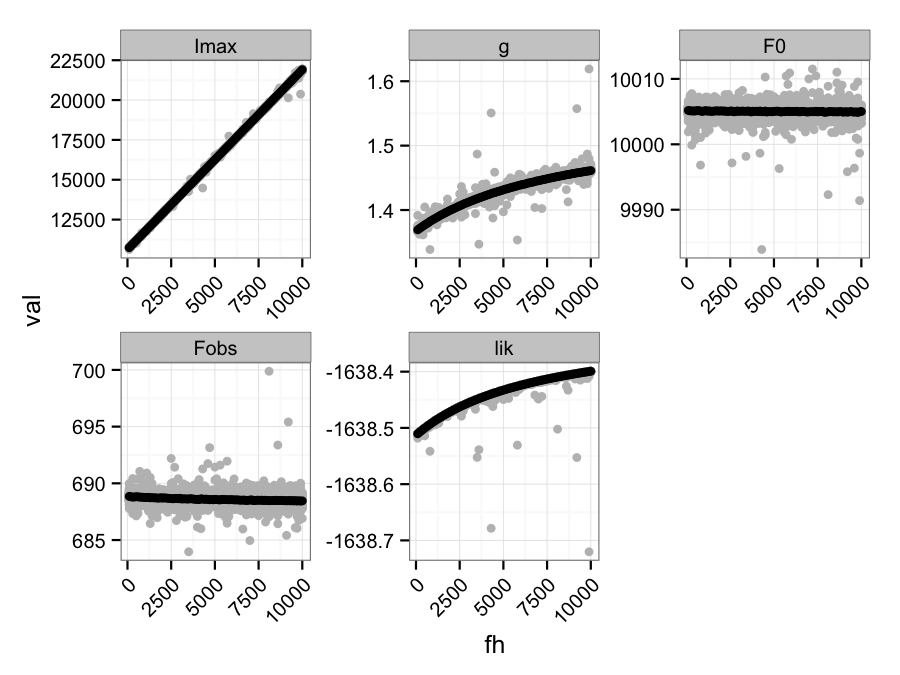
\includegraphics[width=0.8\textwidth]{figure/feeding-1} \hfill{}

\caption[Feeding model parameters for \textbf{uninfected} animals as ]{Feeding model parameters for \textbf{uninfected} animals as $f_h$ is varied. Black points show the maximum likelihood parameter estimates.}\label{fig:feeding}
\end{figure}


\end{knitrout}

Before tackling the problem of estimating the feeding parameters jointly with the growth and reproduction parameters, I want to see whether this fitting procedure supports a lower feeding rate for infected \emph{Daphnia}.
As a first pass, I will let all parameters be re-estimated for the uninfected animals, rather than assuming that any of the parameters estimated for the uninfected animals will carry over.
In reality, of course, the initial food abundance and observation error should be the same, at the very least.
Whether $f_h$ and $g$ should also be the same is less clear to me.

Fig. \ref{fig:inf-feeding} shows the results of this feeding.
While $I_{max}$ is definitely much lower for infected animals compared to uninfected animals, the really huge change is the estimates of $g$: whereas $g > 1$ for uninfected animals, for infected animals, feeding rate is nearly independent of size.
This is kind of interesting, actually, although I am not sure what to make of it.
\begin{knitrout}\scriptsize
\definecolor{shadecolor}{rgb}{0.969, 0.969, 0.969}\color{fgcolor}\begin{figure}

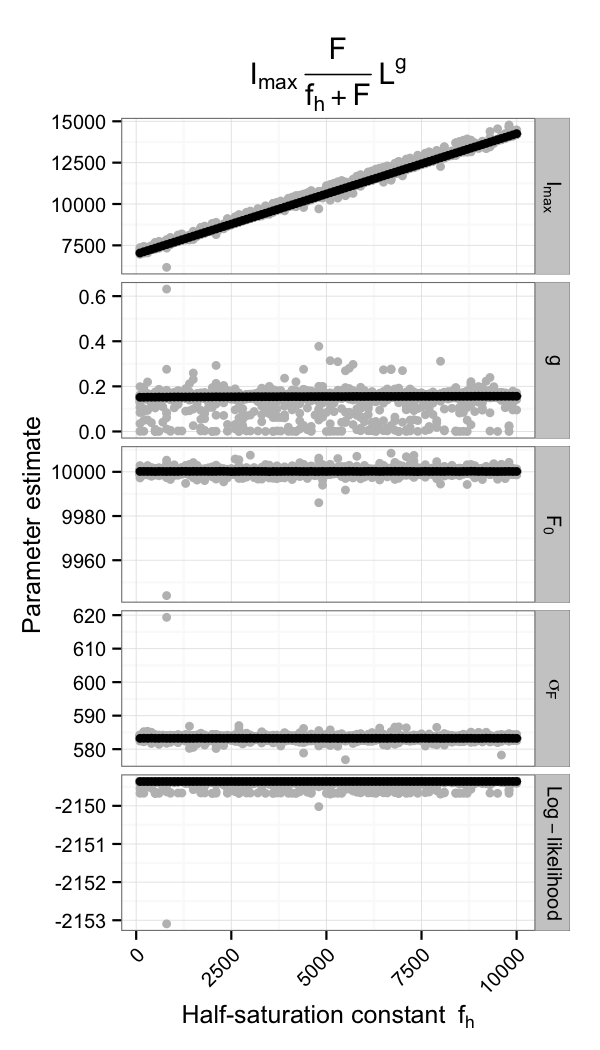
\includegraphics[width=0.8\textwidth]{figure/inf-feeding-1} \hfill{}

\caption[Feeding model parameters for \textbf{infected} animals as ]{Feeding model parameters for \textbf{infected} animals as $f_h$ is varied. Black points show the maximum likelihood parameter estimates for each value of $f_h$.}\label{fig:inf-feeding}
\end{figure}


\end{knitrout}

I also did the fitting fixing $F_0$, $\sigma_F$, and $g$ at the same values as for uninfected animals, so the only parameter I was estimating was $I_{max}$.
In this case, you see an even larger reduction in the estimate of $I_{max}$ between uninfected and infected individuals (Fig. \ref{fig:Imax-comp}).
The likelihood of the $I_{max}$-only model is about 20 log-likelihood units worse than the model where all of the parameters were estimated.
\begin{knitrout}\scriptsize
\definecolor{shadecolor}{rgb}{0.969, 0.969, 0.969}\color{fgcolor}\begin{figure}

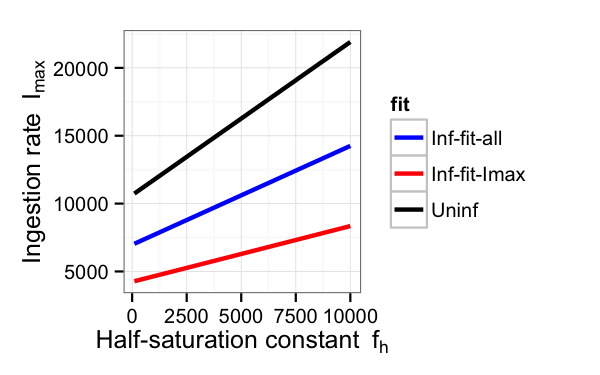
\includegraphics[width=0.7\textwidth]{figure/Imax-comp-1} \hfill{}

\caption[Estimates of ]{Estimates of $I_{max}$ as $f_h$ varies for uninfected animals (black line), for infected animals when all feeding parameters are estimated simultaneously (blue), and for infected animals when $g$ takes the same value as for uninfected animals (red).}\label{fig:Imax-comp}
\end{figure}


\end{knitrout}

Another possibility considered by Spencer is that feeding rate in infected animals is also affected by spore load.
The model he uses, and that I will consider as well, is
\begin{equation*}
\frac{dF}{dt} = -I_{max} \frac{F}{f_h+F} L^g \exp\left(-a\frac{Z}{L^h}\right),
\end{equation*}
where $Z$ is the spore load, $h$ scales body length, and $a$ is the reduction in feeding as the spore load per unit of body size increases.
There is one problem that I don't know how Spencer dealt with, which is how to treat individuals that were exposed but were sacrificed too young to know whether they were infected or not (and were not even checked for spores).
There are two ways to deal with them: either ignore them and only include individuals that were counted, or to treat them all as zeros.
I will try both ways.

For the first attempt, I drop all individuals with NA spore counts.
I estimated $I_{max}$, $a$, and $h$ for a range of $f_h$ values.
I did not attempt to estimate $g$ here, by fixed it at the value estimated for uninfected animals.
The reason for this is that the only infected animals that were counted were fairly large (and thus not growing much).
The lack of variation in size among clearly infected animals makes $g$ nearly impossible to estimate.
Focusing only on parameter sets with log-likelihoods within 1 units of the best-fitting dataset, you can see that the estimates are pretty consistent for a given $f_h$ value (Fig. \ref{fig:spore-dep-feeding}).
Moreover, as $f_h$ increases, the estimates of $a$ and $h$ are basically constant, while $I_{max}$ increases linearly.
The highest likelihood occurs for very small values of $f_h$, though the likelihood difference is small.
The likelihood of this model cannot be compared against the likelihood of the model that did not include spore-dependent feeding reductions because all animals with NA spore counts were dropped here.

\begin{knitrout}\scriptsize
\definecolor{shadecolor}{rgb}{0.969, 0.969, 0.969}\color{fgcolor}\begin{figure}

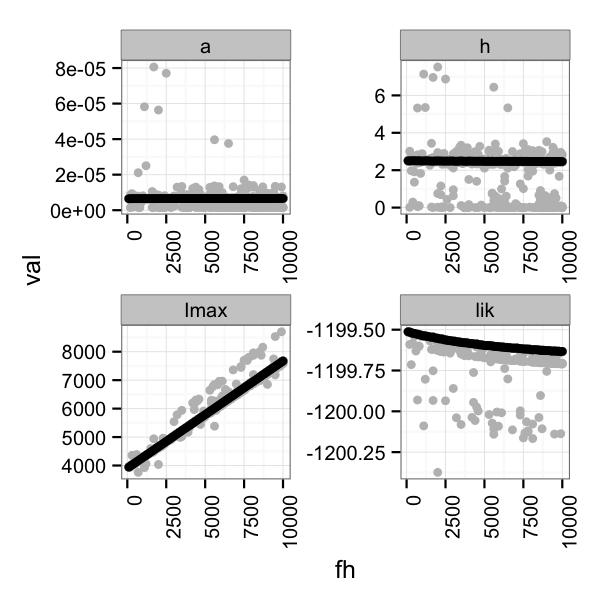
\includegraphics[width=0.8\textwidth]{figure/spore-dep-feeding-1} \hfill{}

\caption[Spore-dependent feeding model parameters for infected animals as ]{Spore-dependent feeding model parameters for infected animals as $f_h$ is varied. Black points show the maximum likelihood parameter estimates for each value of $f_h$. For this fitting, all individuals with NA spore counts were dropped.}\label{fig:spore-dep-feeding}
\end{figure}


\end{knitrout}

If I treat all of the young exposed individuals as infected, but with 0 spore counts instead, the results are quite different.
Comparing Figs. \ref{fig:spore-dep-feeding} and \ref{fig:spore-dep-feeding-2}, you can see that all three parameters ($a$, $h$, and $I_{max}$ increase in value quite a lot when you assume that all of the individuals with NA spore counts are actually infected and have 0 transmission stage spores.
However, although the best-fitting parameter sets have the same values of $a$ and $h$ as $f_h$ increases, there is much more spread around each estimate.
That is, a much greater range of parameter values have nearly equal likelihoods.
That said, I think, in the end, that the parameter estimates shown in Fig. \ref{fig:spore-dep-feeding-2} are the better ones to use.
This is because $Z$ is only considering mature transmission spores, so if you assume that all of the young animals are infected but with 0 transmission spores, then this is the right thing to do.
It also seems reasonable to assume 100\% infection success, given that all of the exposed animals that were sacrificed after day 12 were infected.

\begin{knitrout}\scriptsize
\definecolor{shadecolor}{rgb}{0.969, 0.969, 0.969}\color{fgcolor}\begin{figure}

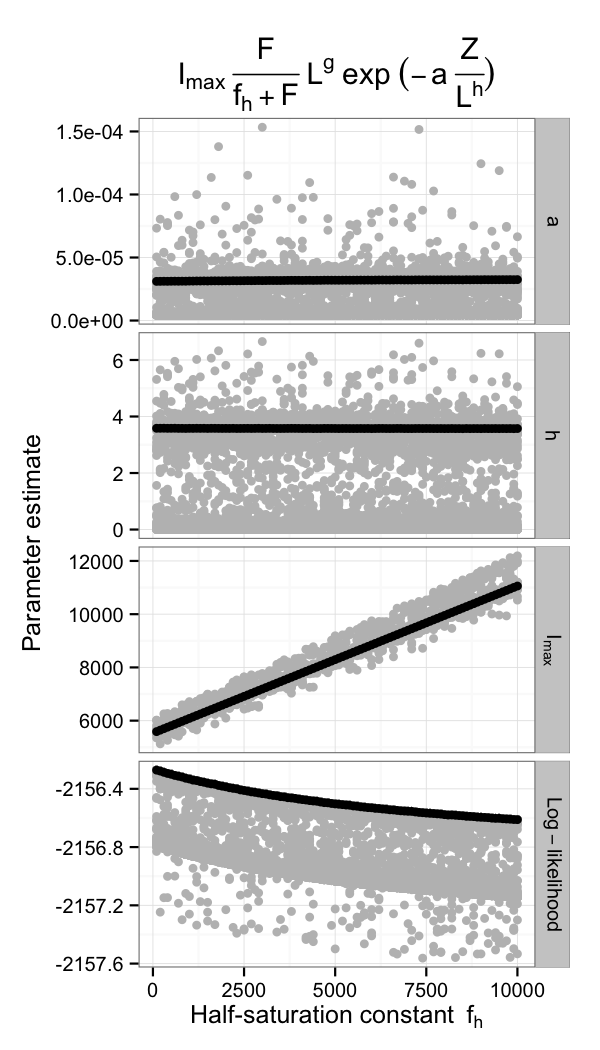
\includegraphics[width=0.8\textwidth]{figure/spore-dep-feeding-2-1} \hfill{}

\caption[Spore-dependent feeding model parameters for infected animals as ]{Spore-dependent feeding model parameters for infected animals as $f_h$ is varied. For this fitting, all individuals with NA spore counts were assumed to have a spore count of 0. Black points show the maximum likelihood parameter estimates for each value of $f_h$.}\label{fig:spore-dep-feeding-2}
\end{figure}


\end{knitrout}

The issue is whether this spore-dependent feeding model has a significantly higher likelihood than the simpler model than assumed spore-independent feeding (the model that fit only $I_{max}$), since that model was also fitted to the data for all exposed individuals.
The likelihood of the spore-dependent model is higher, of course, because there are more free parameters.
Based on AIC$_{\text{c}}$ differences, the spore-dependent model is preferred over the spore-independent model: the AIC$_{\text{c}}$ of the spore-dependent model is 16 units smaller than the AIC$_{\text{c}}$ of the spore-independent model, suggesting that the spore-independent model is about 0.0002 times as probable as the spore-dependent model.
This conclusion is also supported by a likelihood ratio test, which suggests that the probability of such a likelihood difference occurring by chance as less than $10^{-4}$.



I can also compare the observed data against model predictions for both infected and uninfected animals.

In particular, I will calculate the expected clearance rate for every animal, based on the best-fitting model (assuming $f_h = 5000$), and compare that prediction against the observed clearance rate.
For this model, the parameter estimates were $g=1.43$, $a=3.2\times10^{-5}$, and $h=3.56$, with $I_{max}=16264$ for uninfected animals and $I_{max}=8293$ for infected animals.
Clearance rate was calculated as $\log\left(\frac{F(0)}{F(t)}\right)~\frac{V}{t}$, where $V$ is the volume of beaker, $t$ is the total time of the trial, and $F(0)$ and $F(t)$ give the concentration of food at time 0 and time $t$, respectively.
Fig. \ref{fig:clearance-thru-time} shows how clearance rate changes across the age of the individuals.
You can see clearly that infected animals feed at a lower rate than uninfected animals.
The model tends to underpredict feeding rate early in life for both sick and healthy animals, and the variance in the expected feeding rate among animals of the same age is much smaller than the observed variance.
However, the predicted variance is higher than what is observed here because I am not taking account of the observation error - I could have plotted error bars around each of the predicted points based on the observation error in both initial and final food concentrations.

\begin{knitrout}\scriptsize
\definecolor{shadecolor}{rgb}{0.969, 0.969, 0.969}\color{fgcolor}\begin{figure}

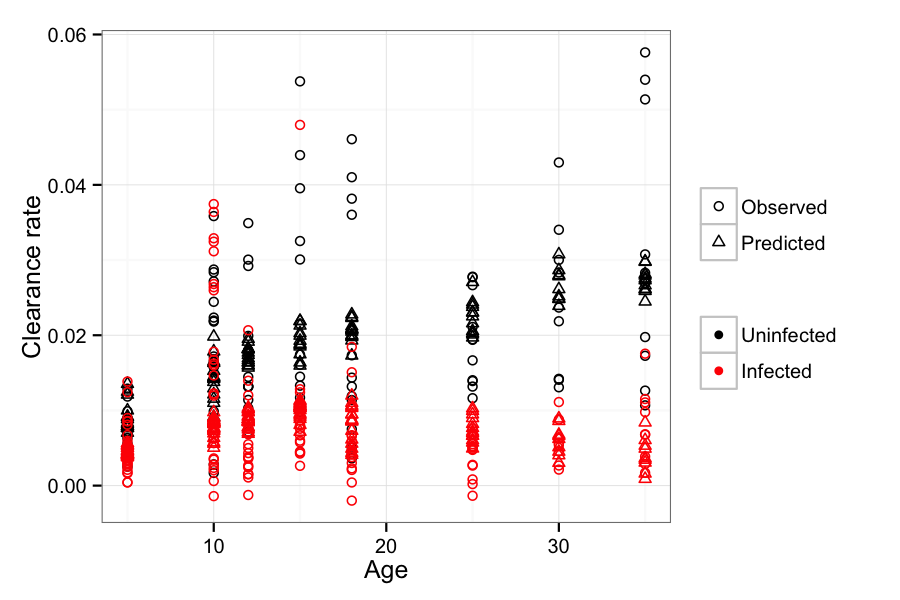
\includegraphics[width=\linewidth]{figure/clearance-thru-time-1} \hfill{}

\caption[Comparing observed versus predicted clearance rates for both infected and uninfected animals across the lifespan, assuming the best fit parameter values]{Comparing observed versus predicted clearance rates for both infected and uninfected animals across the lifespan, assuming the best fit parameter values.}\label{fig:clearance-thru-time}
\end{figure}


\end{knitrout}

The last thing that I want to do is to see if my feeding model does a better job fitting the data than does the parameter estimates reported by Spencer.
Let's hope so, since I spent so much time fitting the data!
To evaluate this, I will plot the observed versus predicted clearance rates for each individual and then calculate an $R^2$ value based on the difference between each individual datapoint and the one-to-one line.
I will do this for my model, and also for Spencer's model, which predicted the clearance rates as
\begin{align}
f_U~L^g & \text{for uninfected animals}, \\
f_I~L^g~\exp\left(-a~\frac{Z}{L^h}\right) & \text{for infected animals},
\end{align}
with $f_u = 0.0126$, $g=1.3704$, $f_i=0.0061$, $a=0.0205$, and $h=2.6420$.
What you notice right away from Fig. \ref{fig:Clay-vs-Spencer} is that the predicted clearance rate is zero for many of the infected animals, under Spencer's model.
This is because the estimate of $a$ that Spencer reports is much, much higher than my estimate (0.0205 vs. $3.2\times10^{-5}$).
Because of this, the $R^2$ for my model is much higher than Spencer's, 0.36 versus 0.28.
If you focus only on the uninfected animals, our models are equally good (0.257 for my model versus 0.258 for Spencer's model).
Thus, I feel confident moving forward with my model for feeding, with the caveat that I still don't know what the appropriate value of $f_h$ is.
To address this, I will fit growth and reproduction trajectories, with algae having their own dynamics, to see whether this helps at all with tightening up the estimates of both $f_h$ and also $v$, the energy conductance.
I will begin with generating simulated datasets, as before, and fitting the DEB models to those datasets.
It is my hope that the dynamic food resource will reveal both the value of $f_h$ (because algal abundance will drop low enough for it to matter) and $v$ (because dynamic food will cause more dynamism in the value of $E$, thereby making the value of $v$ more important).

\begin{knitrout}\scriptsize
\definecolor{shadecolor}{rgb}{0.969, 0.969, 0.969}\color{fgcolor}\begin{figure}

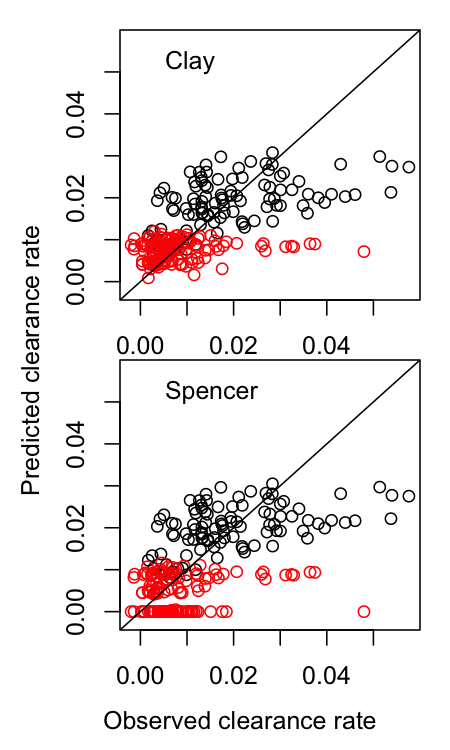
\includegraphics[width=0.6\textwidth]{figure/Clay-vs-Spencer-1} \hfill{}

\caption[Comparing the fits of my model to Spencer's model by plotting observed clearance rates against model-predicted clearance rates for both uninfected and infected animals]{Comparing the fits of my model to Spencer's model by plotting observed clearance rates against model-predicted clearance rates for both uninfected and infected animals.}\label{fig:Clay-vs-Spencer}
\end{figure}


\end{knitrout}

\end{document}
